\documentclass[a4paper, 12pt]{article}

\usepackage{babel}
\usepackage{enumitem}
\usepackage{times}
\usepackage{graphicx}
\usepackage{geometry}
	\geometry{left = 4cm, top = 4cm, right = 3cm, bottom = 3cm}
\usepackage{float}
\usepackage{setspace}
	\setstretch{1.5}


\begin{document}
\title{\huge\textbf{Tugas Praktikum Pemrograman II}}
\date{}

\maketitle


\begin{figure}[!ht]
\begin{center}

\includegraphics[width = 5cm, height = 4.5cm]{gambar/logo.png}
\end{center}
\end{figure}

\begin{center}
\vspace{1cm}
Disusun oleh :\\
Syabriena Putri Veriane\\
D4 TI 2B\\
1.18.4.094\\
\vspace{1cm}
\textbf{PROGRAM DIPLOMA IV POLITEKNIK POS INDONESIA} \linebreak
\textbf{POLITEKNIK POS INDONESIA} \linebreak
\textbf{BANDUNG}\linebreak
\textbf{2019}

\end{center}

\thispagestyle{empty}

\clearpage
\setcounter{page}{1}

\begin{center}
\title{\LARGE \bf Mengenal Python dan Anaconda}
\end{center}

\appendix
\section{Teori}

\section*{\normalsize 1. Sejarah dan Perbedaan}

\hspace {\parindent} Python diciptakan oleh Guido Van Rossum di Centrum Wiskunde and Informatica, Belanda tahun 1990. Guido lanjut membuat bahasa python di Corporation for National Research Initiative di Amerika tahun 1995. Pada pembuatan ini kemudian dirilis beberapa versi python.

Nama bahasa pemrograman ini diambil dari nama grup komedi di Inggris yang digemari oleh Guido yaitu "Monty Python". Bahasa pemrograman ini terinspirasi dari bahasa pemrograman ABC. Python bersifat open source yang berarti bahasa pemrograman ini masih bisa dikembangkan oleh orang yang ingin mengembangkannya.

Pada tahun 2001, terbentuklah Organisasi Python yang bernama Python Software Foundation(PSF)nyang merupakan organisasi yang dibuat khusus untuk hak intelektual Python. Bahasa pemrograman python sendiri setelah dirilis memiliki beberapa versi. Setiap versi memiliki perbedaan, berikut adalah perbedaan python versi 2 dan versi 3 :
\begin{enumerate}[label=\alph*.]
\item Syntax untuk mencetak teks
Pada Python 2 : perintah cetak tidak harus menggunakan kurung tetapi menggunakan kurung juga bisa.
Contoh :
print "Kayak gini bisa"

Pada Python 3 : perintah cetak harus menggunakan kurung.
Contoh :
print ("Kayak gini loh")

\item Syntax untuk meminta inputan
Pada Python 2 : perintah input user menggunakan perintah raw\textunderscore input.
Contoh : 
nama = raw\textunderscore input('Masukkan nama')

Pada Python 3 : perintah input user menggunakan perintah input.
Contoh :
nama = input('Masukkan nama')

\item Hasil dari operator pembagian
Pada Python 2 :
print "3 /2 =", 3/2\\
print "3 // 2 =", 3//2\\
print "3 / 2.0 =", 3/2.0\\

hasilnya
3 / 2 = 1.5\\
3 // 2 = 1\\
3 / 2.0 = 1.5\\
3 // 2.0 = 1.0\\

Pada Python 3 hasilnya :
3 / 2 = 1.5\\
3 // 2.0 = 1\\
3 / 2.0 = 1.5\\
3 // 2.0 = 1.0\\

\end{enumerate}

\section*{\normalsize 2. Implementasi Penggunaan Python pada Perusahaan Dunia}
\hspace{\parindent}Perusahaan besar pengguna python adalah perusahaan google. Google menggunakan pemrograman python untuk webnya dengan menggunakan library python, tools, dan framework. Python menjadi bahasa yang digunakan pada Google App Engine nya, dan programmer menggunakan python untuk membangun sistem administrasi, format package internal google, dan aplikasi penampil kode. Selain itu, python digunakan juga pada platform youtube. Pada youtube, python digunakan untuk menampilkan video, mengontrol website, dan akses data.

%SECTION 2-----------------------------------------------------------------------------------------------------------------------<

\section{Instalasi}
\begin{enumerate}

\item Instalasi Python

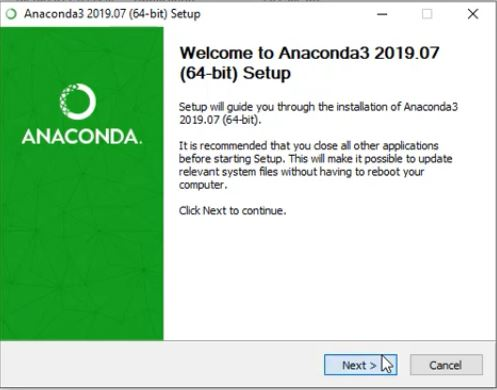
\includegraphics{gambar/1_1.jpg}
Klik Next\\

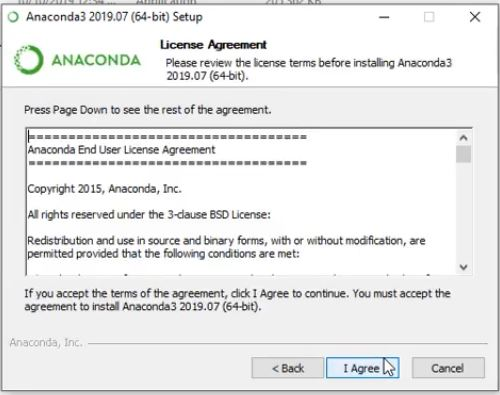
\includegraphics{gambar/1_2.jpg}
Klik Agree\\

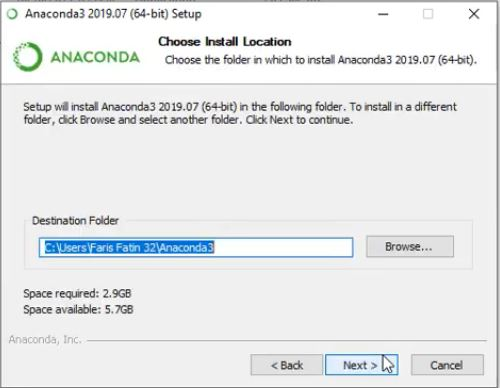
\includegraphics{gambar/1_3.jpg}
Pilih direktori install\\

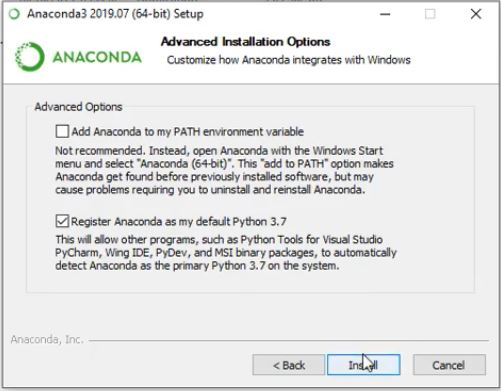
\includegraphics{gambar/1_4.jpg}
Klik install\\

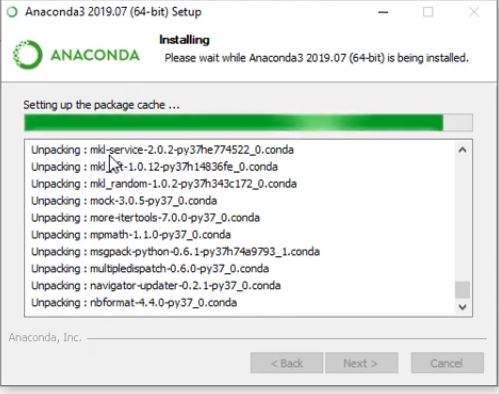
\includegraphics{gambar/1_5.jpg}
Tunggu installan hingga selesai\\

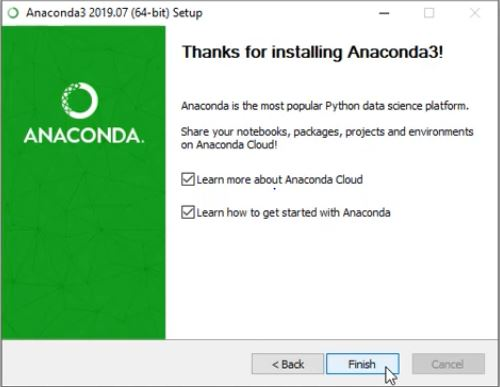
\includegraphics{gambar/1_6.jpg}
Selesai\\



\item Instalasi pip

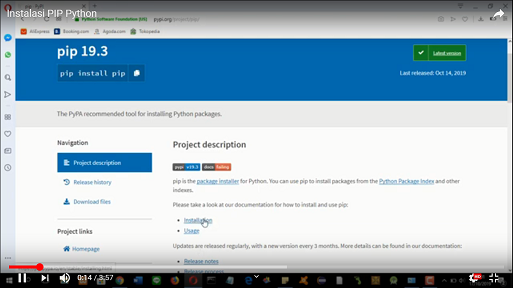
\includegraphics{gambar/pip_1.png}
Buka web pip.py\\

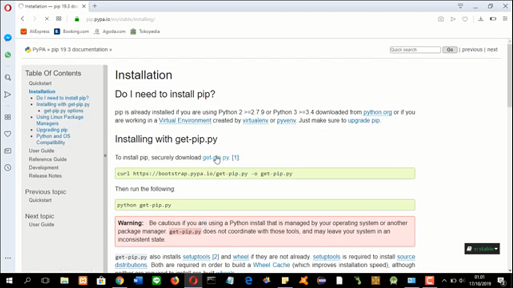
\includegraphics{gambar/pip_2.png}
Klik get-pip.py\\

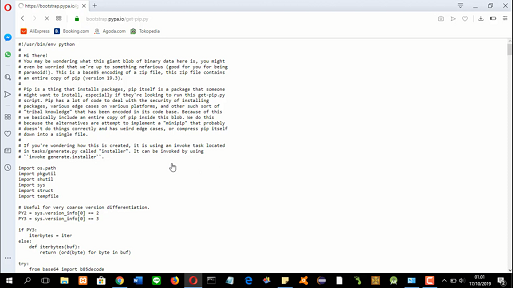
\includegraphics{gambar/pip_3.png}
Download file get-pip.py\\

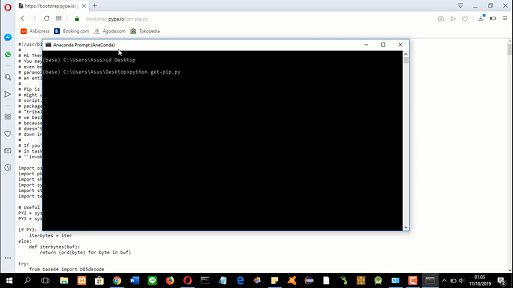
\includegraphics{gambar/pip_4.png}
Buka cmd, ketik perintah "python get-pip.py". Tunggu instalasi berjalan\\

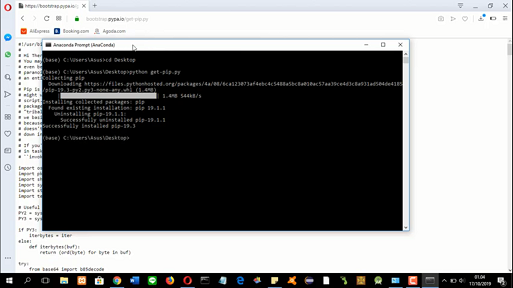
\includegraphics{gambar/pip_5.png}
Install selesai\\
Link :\\
https://www.youtube.com/watch?v=YI2NjDYU\textunderscore dU


\item Cara Setting Environtment

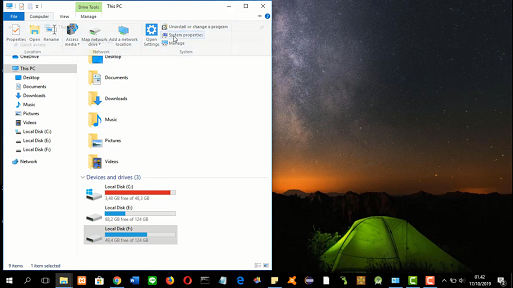
\includegraphics{gambar/ev_1.png}
Buka system properties\\

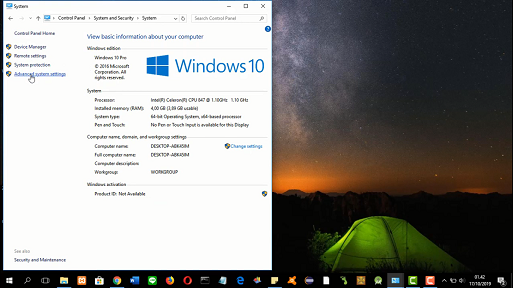
\includegraphics{gambar/ev_2.png}
Buka Advance system setting\\

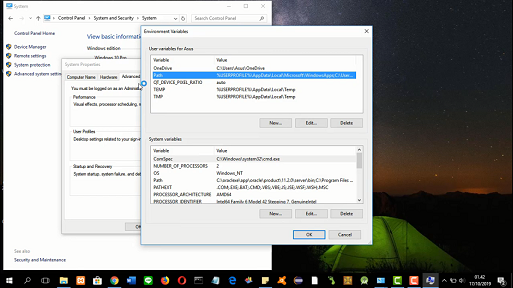
\includegraphics{gambar/ev_3.png}
Klik environtment variables\\

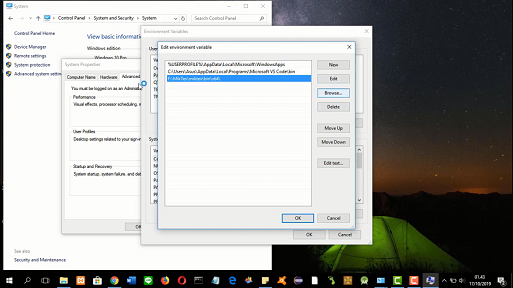
\includegraphics{gambar/ev_4.png}
Klik environtment path python\\
Link :\\
https://www.youtube.com/watch?v=KMGWeEjlFP8


\item Mencoba Enterpreter CLI

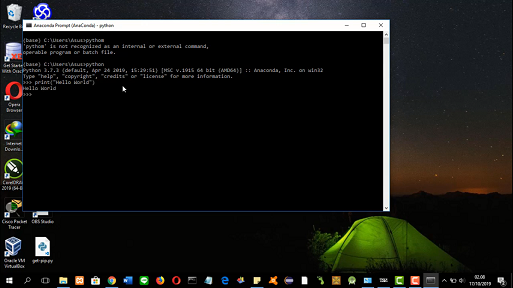
\includegraphics{gambar/cli.png}
Buka CLI/cmd, lalu ketik ("Hello World")\\
Link :\\
https://www.youtube.com/watch?v=mCF8Jdcyx8k


\item Menjalankan dan Update Anaconda Spyder

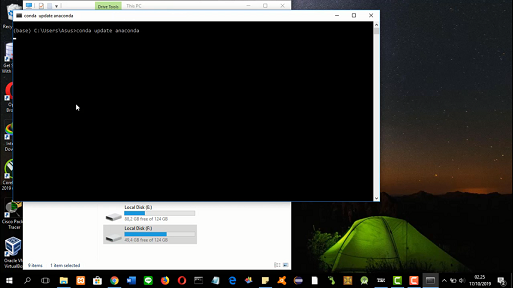
\includegraphics{gambar/upd1.png}
Buka CLI/cmd, lalu ketik "conda update anaconda"\\

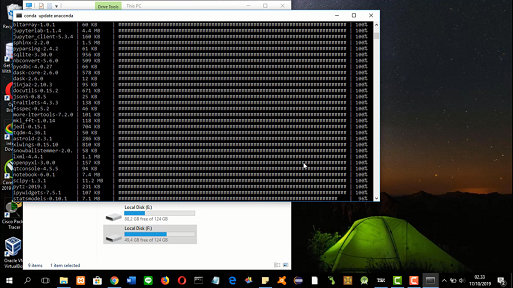
\includegraphics{gambar/upd2.png}
Conda otomatis download dan update\\

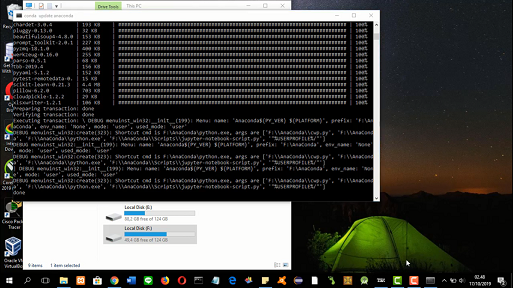
\includegraphics{gambar/upd3.png}
Update selesai\\
Link :\\
https://www.youtube.com/watch?v=ecbBPO57l\textunderscore E


\item Cara Menjalankan Script Hello World di Spyder


\includegraphics{gambar/hello.png}
Ketik ("Hello World") lalu run, hasil akan muncul dalam console\\
Link video :\\
https://www.youtube.com/watch?v=WBal7rotqww


\item Cara Menggunakan Variabel Explorer di Spyder

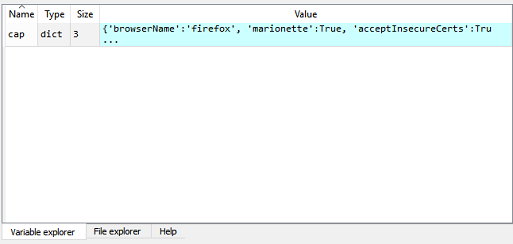
\includegraphics{gambar/var.png}
Variabel Explorer digunakan untuk mencari apa saja nama, type, dan value dari variabel yang digunakan spyder. Bisa juga untuk mengedit dan mengubah variabel.\\
\end{enumerate}

\section{identasi}
\begin{enumerate}
\item Pengertian
Identasi yaitu penulisan paragraf yang menjorok kedalam. Dalam bahasa pemrograman python, identasi digunakan sebagai tatacara menulis dan tidak memakai tanda kurung.

\item{Jenis-Jenis Error}

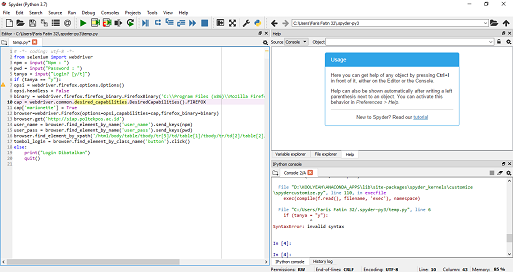
\includegraphics{gambar/identasi1.png}
Eror ini disebabkan identasi yang kurang benar.\\


\item{Cara Membaca Error}

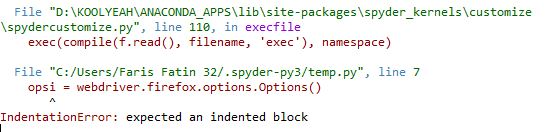
\includegraphics{gambar/identasi3.jpg}
Opsi = webdriver.firefox.Options() berarti eror pada bagian ini.
IndentationError: expected an indented block berarti error pada line tadi dan disebabkan oleh identasi.\\


\item{Cara Menangani Error}

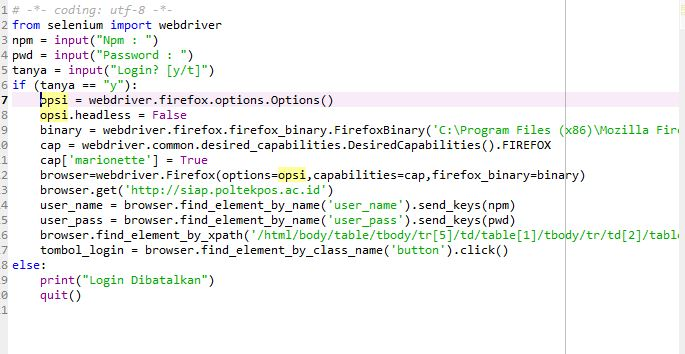
\includegraphics{gambar/identasi4.jpg}
Cara menangani error dengan memberikan identasi ke line yang belum teridentasi.\\

\end{enumerate}
\end{document}

